\section{Metodologia} \label{Metodologia}
% TODO adicionar uma forma de comparar um hardware convencional(asics)
Serão apresentados quatro cenários neste trabalho, que visam comparar o desempenho e capacidade de fluxo de dados na rede. Seram analizados roteadores \ac{ASIC} assim como roteadores rodando linux, com o intuito de comparar o desempenho da rede. 

O cenário I representará um ambiente de controle, ou seja, não possuirá roteadores. Ambos computadores se comunicaram utilizando um \textit{switch} TP-Link de 100 Megabit de banda. O cenário II e III será um ambiente com um roteador linux entre os computadores, sendo que no cenário II o roteador terá grande poder computacional comparado com o cenário III onde ele terá baixo poder computacional. Já no cenário IV será testado um roteador \ac{ASIC} rodando \textit{firmware} customizado para coleta de métricas.

Cada cenário será testado com uma série de testes de performance e estabilidade. Será também levado em conta a difença de consumo de recursos em ambos cenários. A ferramente principal desses testes será o iPerf3, que será configurado para enviar datagramas UDP de diversos tamanhos, durante um perido de 30 segundos 10 vezes.

Tem-se como hipótese que o cenário I terá o melhor desempenho comparado com o restante e que o cenário II e IV teram resultados aproximadamente parecidos. Se espera que no cenário III o desempenho será afetado pela falta de recursos do roteador.
\begin{figure}[H]
    \centering
    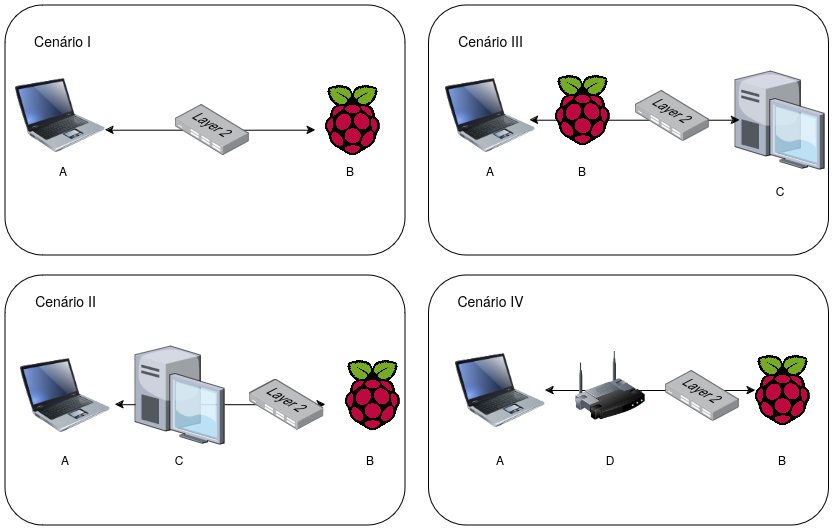
\includegraphics[width=0.9\linewidth]{sources/fig-cenarios.png}
    \caption{Cenários dos testes a serem realizados.}
    \label{fig:cenarios}
\end{figure}


